\section{Zieldefinition}
Das Ziel dieser Untersuchung ist der Betrieb des Langenthaler Standorts der 
Firma Güdel. Dieser erstreckt sich über 4 Gebäude welche alle mit Gas beheizt
werden. Die Untersuchung beinhaltet die Beschaffung der Werkzeuge und 
Arbeitsplätze in der Montage und in den Büros sowie deren Einrichtung wie auch 
ihren Betrieb und der, der Gebäude.

\[\frac{n!}{k!(n-k)!} = \binom{n}{k}\]

\[\sqrt[n]{1+x+x^2+x^3+\dots+x^n}\]
\[\int_0^\infty \mathrm{e}^{-x}\,\mathrm{d}x\]
\[\displaystyle\sum_{i=1}^{10} t_i\]
Die Produktionstätten werden
von der Untersuchung ausgeschlossen da sie im Vergleich zu den restlichen
Arbeitsplätzen ein x-faches an Energie benötigen. Um hier eine effiziente
Untersuchung machen zu können sollten diese Arbeitsplätze separat untersucht
werden.
\newpage
\subsection{Die Gebäude}
\subsubsection{Werk 1}
In diesem Gebäude befinden diverse Büroarbeitsplätze für Konstruktion,
Hardwareplanung, Verkauf, die Finanzabteilung Güdel Schweiz sowie das 
Personalbüro. Desweiteren ist hier auch die Produktion der Getriebe-Einzelteile 
sowie die Schienenfertigung, Härterei und die Lehrwerkstätten der Polymechaniker
Lehrlinge.
\begin{figure}[ht]
    \centering
    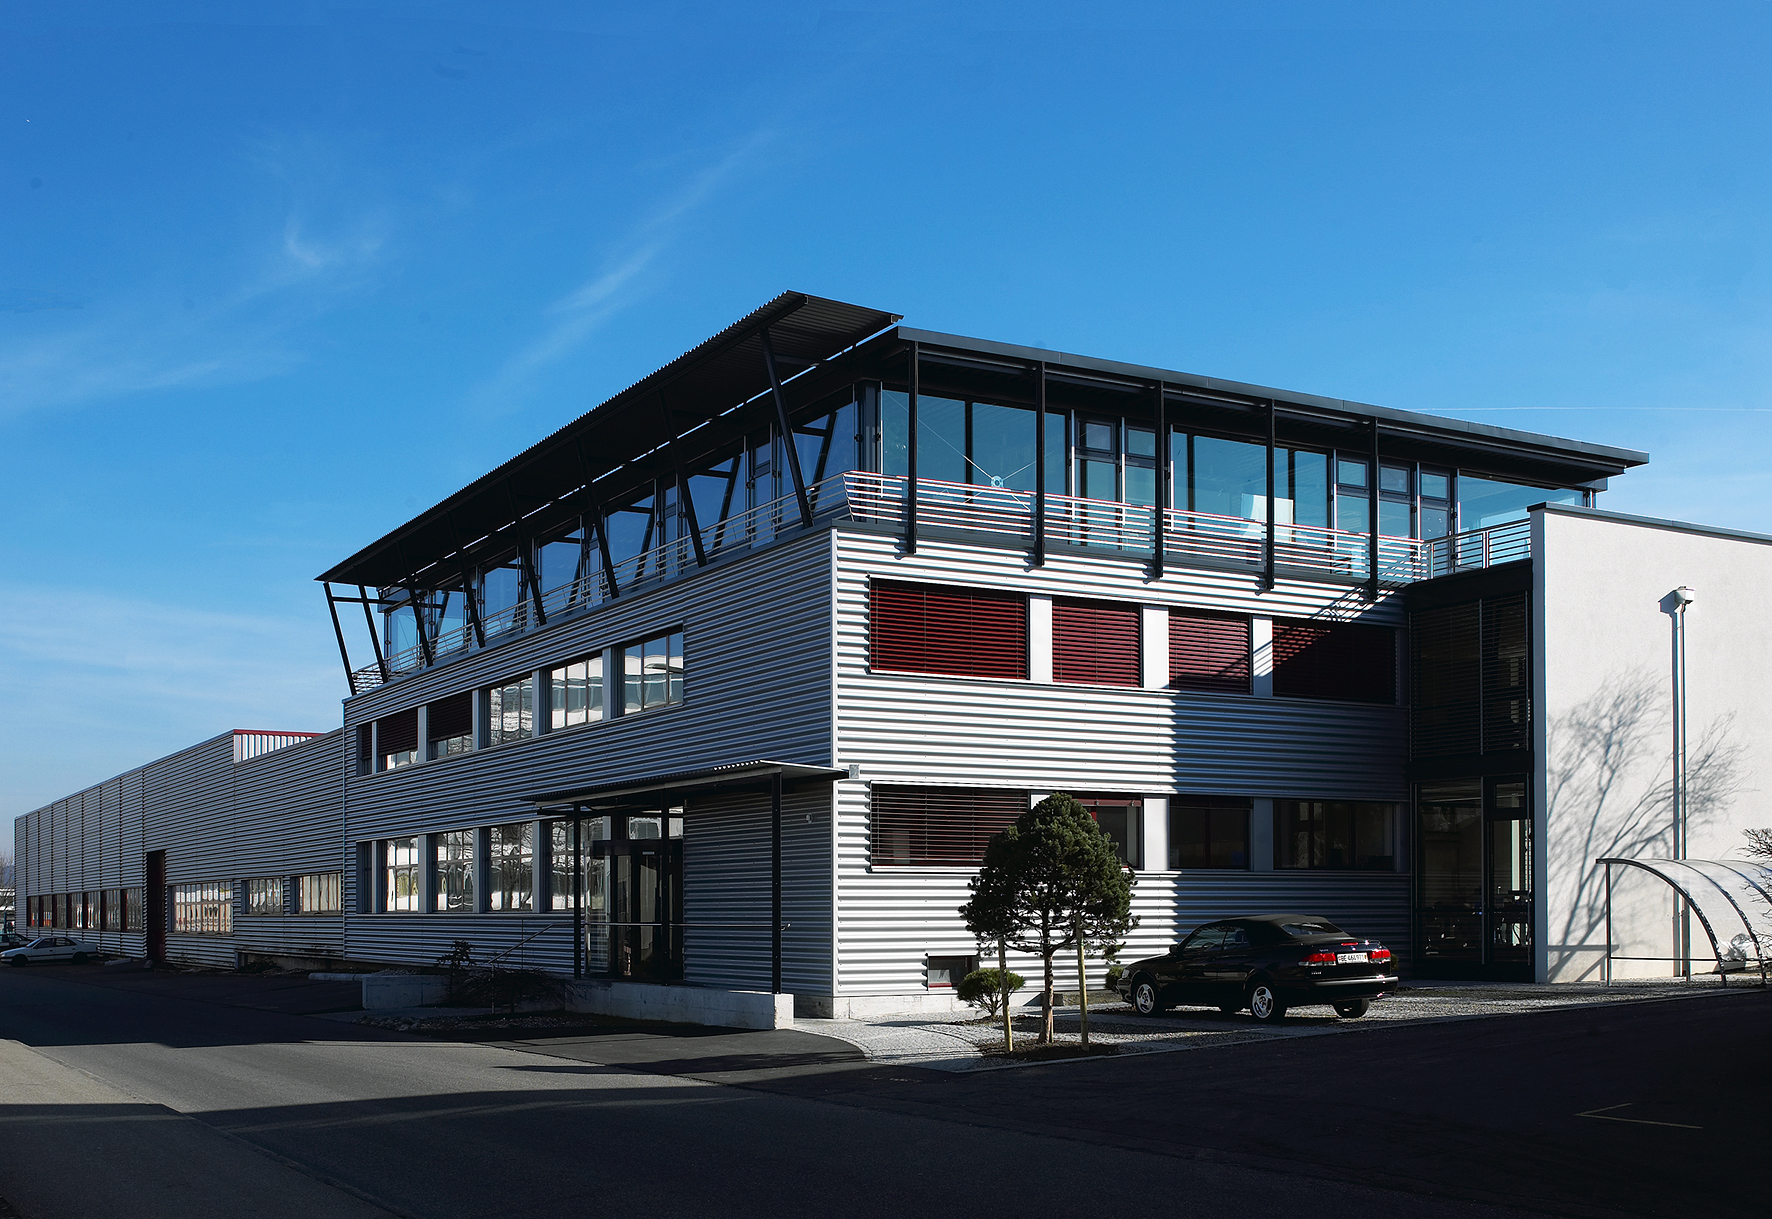
\includegraphics[scale=0.75]{werk_1.jpg}
    \caption{Haupteingang des Werk 1}
\end{figure}
\newpage
\subsubsection{Werk 2}
Das Werk 2 beherbergt hauptsächlich das Lager sowie die Modulmontage. Im
vorderen Teil befinden sich noch die Büros des Supply Chain Management. Im
hinteren Teil sind die R\&D Abteilung und die Lehrwerkstätten der Automatiker zu
finden.
\begin{figure}[ht]
    \centering
    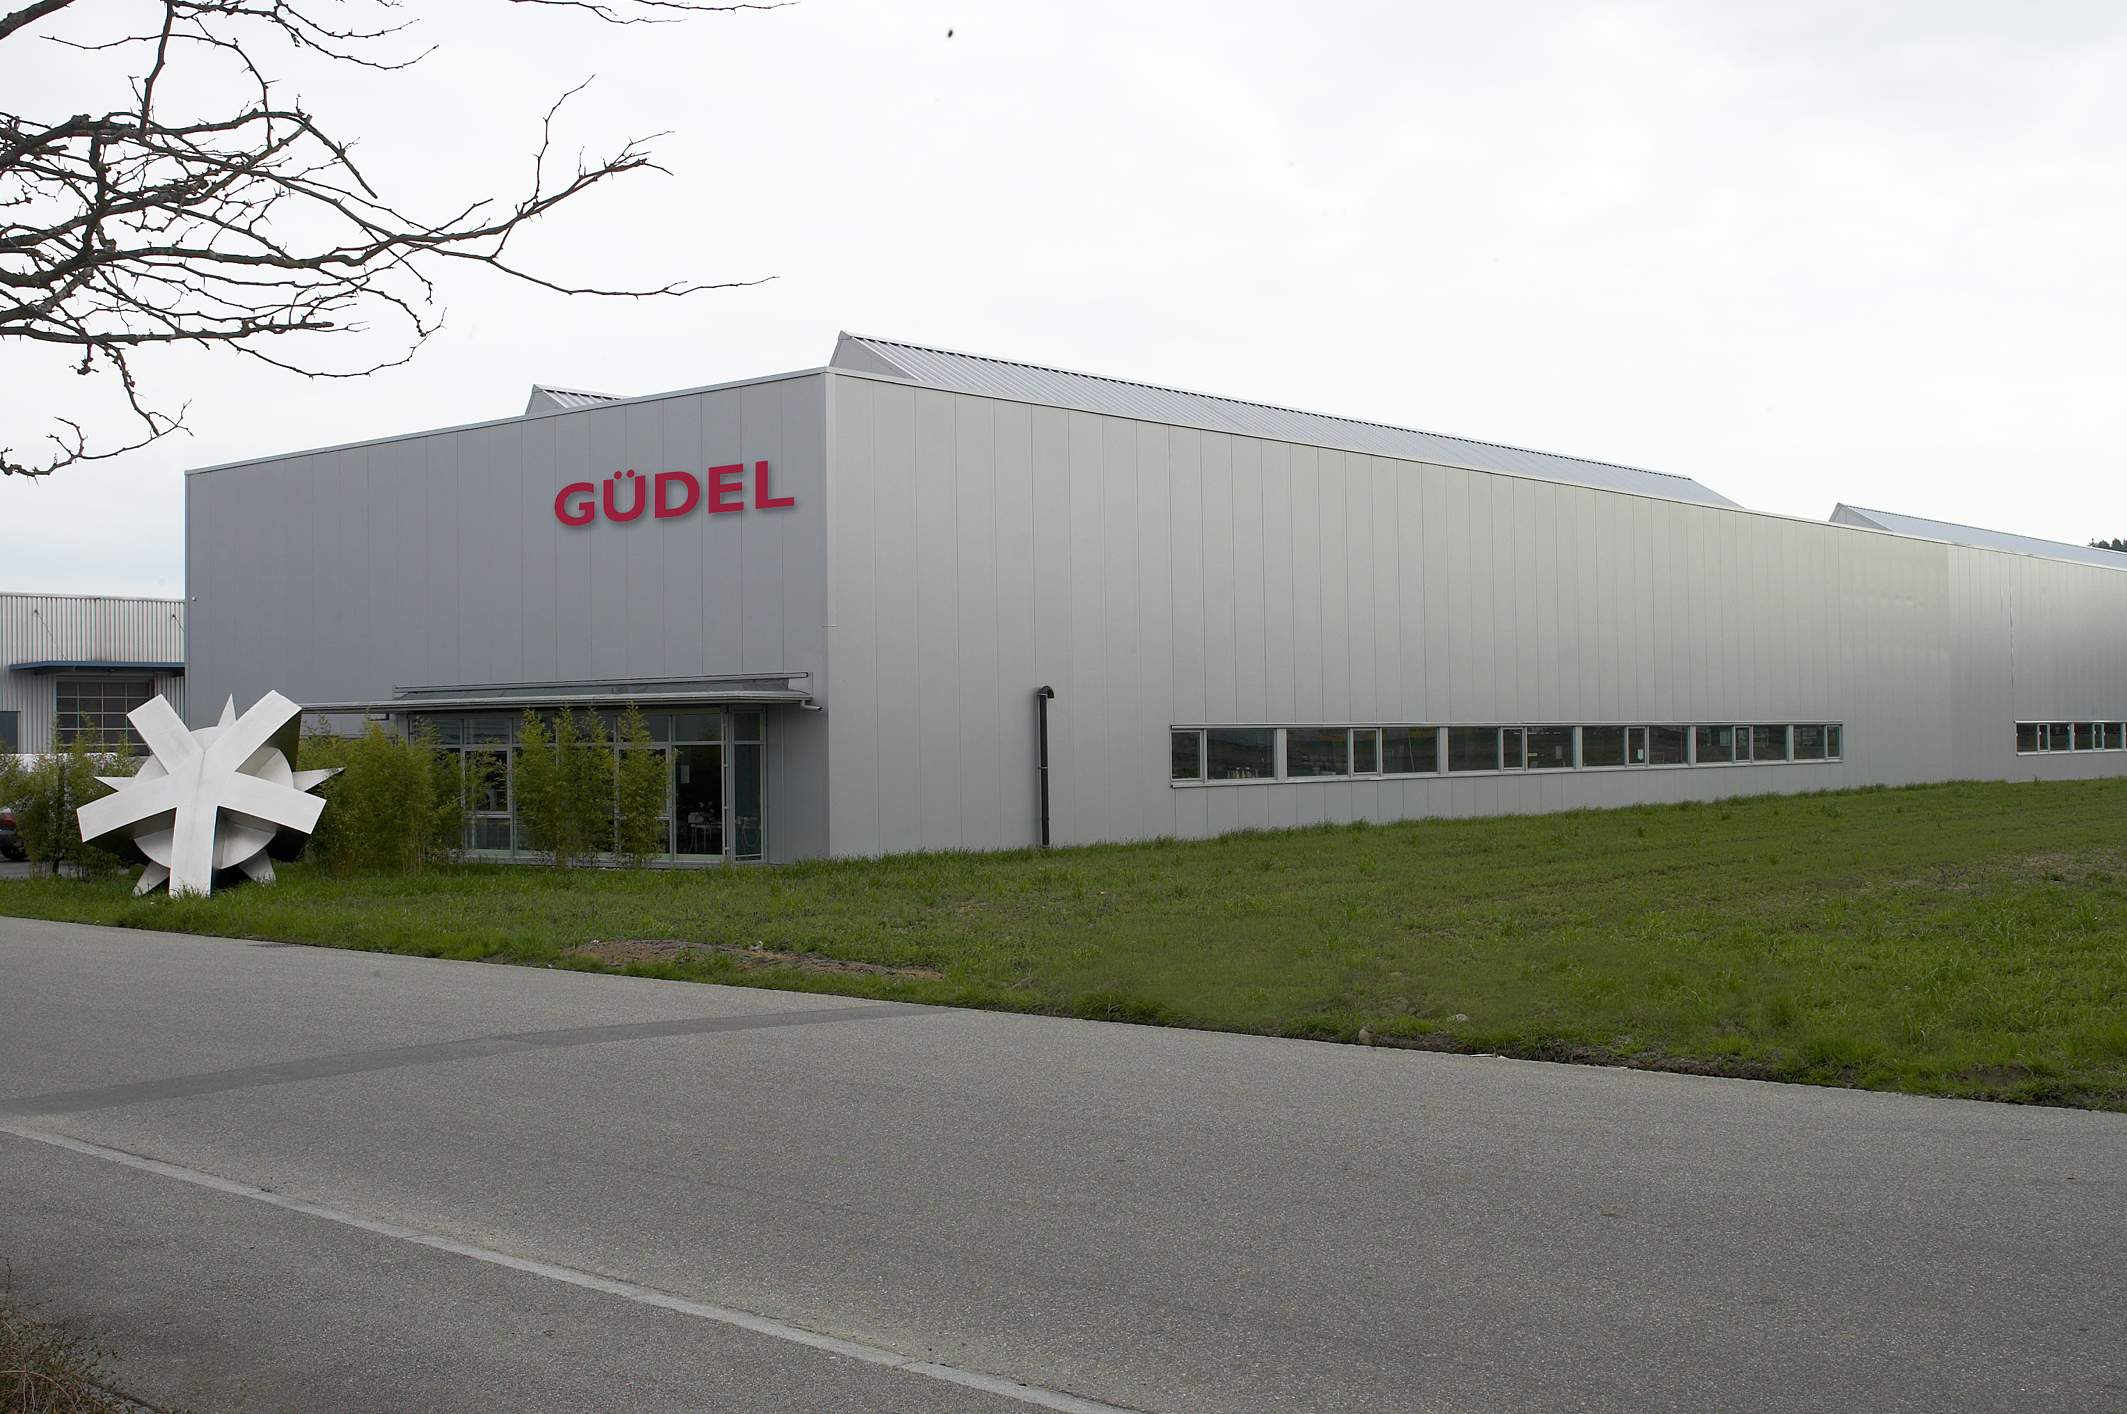
\includegraphics[scale=0.15]{werk_2.jpg}
    \caption{Haupteingang des Werk 2}
\end{figure}

\subsubsection{Werk 3}
Das Werk 3 besteht aus zwei Teilen.\\
Zum einen die Montage- und Produktionshallen
welche die Montagen der Business Units ``Metal Sheet Handling'' und 
``Technologies'' sowie die Grossteilefertigung beherbergen. 
Auch die Büros des Service und der IT Abteilung befinden sich in diesem Teil.
\newpage
Zum anderen aus einem grosser Bürotrakt welcher die diversen Abteilung der Business
Unit ``Metal Sheet Handling'' beinhaltet sowie alle Büroarbeitsplätze der Güdel
Group.
\begin{figure}[ht]
    \centering
    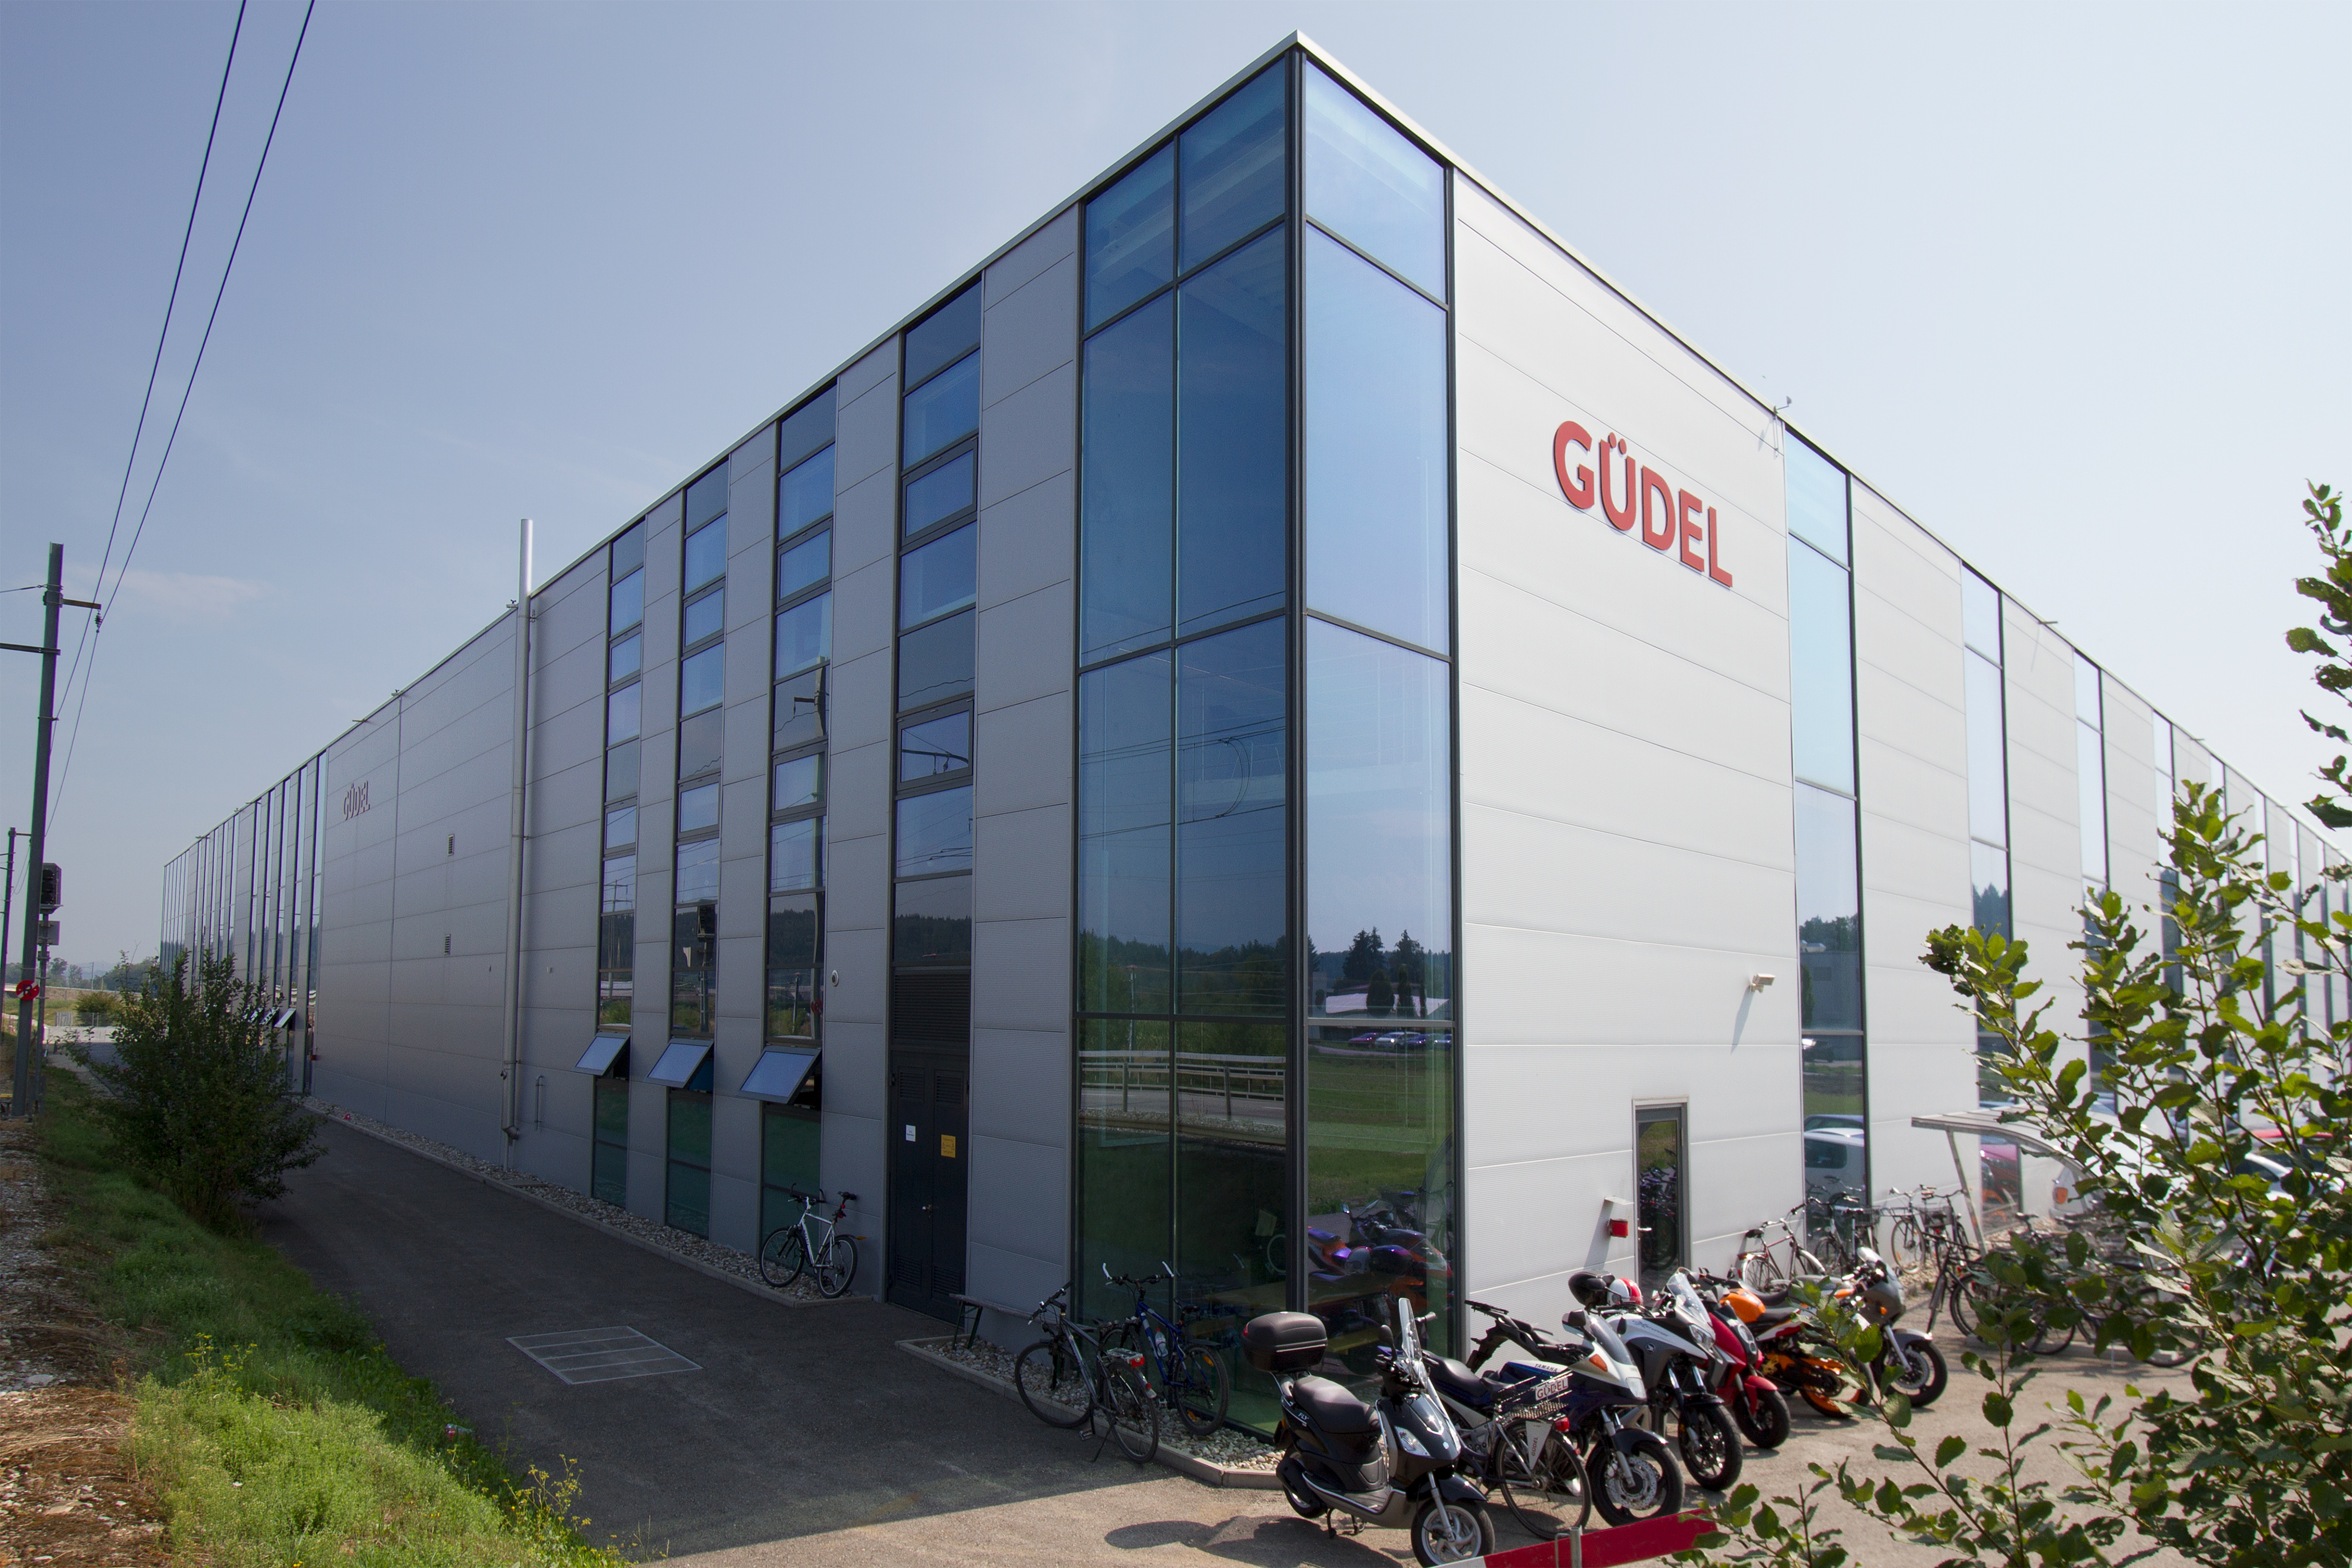
\includegraphics[scale=0.25]{werk_3.jpg}
    \caption{Rückseite des Werk 3}
\end{figure}
\subsubsection{Malerei}
Die Malerei ist im Vergleich zu den anderen Gebäuden relativ klein und
beherbergt nur ein kleines Büro für den Abteilungsleiter und die Lackierräume.

\begin{landscape}

%\begin{sidewaystable}
\section{Ökoinventar}
\vfill
\begin{table}[h]
    \begin{tabular}{ |m{3.5cm}|m{2.5cm}|m{2.5cm}|m{3cm}|m{3cm}|m{3.5cm}| }
\hline
\rowcolor[gray]{0.9}\textbf{Verbrauch/Belastung} & \textbf{Beschaffung} &
\textbf{Lagerung} & 
\textbf{Einrichten} & \textbf{Nutzung/Betrieb} & \textbf{Entsorgung} \\ \hline
Materialverbrauch & Holz, Kunsstoff, Papier & & Werkzeuge, Holz, Alluminium, Papier & Werkzeuge,
Papier & Werkzeuge, Papier \\ \hline
Energieverbrauch & Diesel, Strom, Gas & Strom, Gas & Strom, Gas, Benzin & Strom, Gas
& Strom, Gas, Benzin, Diesel\\ \hline
Umweltbelastung & Abgase & Abgase & Abgase & Abgase
& Abgase, Kunstoffverbrennung, Abfälle \\
\hline
\end{tabular}
\end{table}
\vfill
%\end{sidewaystable}
\end{landscape}

%\begin{sidewaystable}
\begin{landscape}
\section{Bewertung}
\vfill
\begin{table}[h]
    \begin{tabular}{ |m{3.5cm}|m{2.5cm}|m{2.5cm}|m{3cm}|m{3cm}|m{3.5cm}| }
\hline
\rowcolor[gray]{0.9}\textbf{Verbrauch/Belastung} & \textbf{Beschaffung} &
\textbf{Lagerung} & 
\textbf{Einrichten} & \textbf{Nutzung/Betrieb} & \textbf{Entsorgung} \\ \hline
Materialverbrauch & \cellcolor{orange}Holz, Kunsstoff, Papier & \cellcolor{green}&
\cellcolor{yellow}Werkzeuge, Holz, Alluminium, Papier & \cellcolor{orange}Werkzeuge,
Papier & \cellcolor{yellow}Werkzeuge, Papier, Lösungsmittel \\ \hline
Energieverbrauch & \cellcolor{yellow}Diesel, Strom, Gas &
\cellcolor{orange}Strom, Gas & \cellcolor{yellow}Strom, Gas, Benzin &
\cellcolor{red}Strom, Gas
& \cellcolor{orange}Strom, Gas, Benzin, Diesel\\ \hline
Umweltbelastung & \cellcolor{orange}Abgase, Kunstoffabfälle & \cellcolor{yellow}Abgase &
\cellcolor{yellow}Abgase & \cellcolor{red}Abgase
& \cellcolor{red}Abgase, Kunstoffverbrennung, Abfälle, Quecksilber \\
\hline
\end{tabular}
%\end{sidewaystable}
\end{table}
\vfill
\end{landscape}

\section{Massnahmen}
Am grössten ist der Strom- und Gasverbrauch wärend der Nutzung. Der
Stromverbrauch kann hier nur insofern gesenkt werden als das die Leute die
Geräte die sie nutzen regelmässig in den Standby Modus versetzen. Hier wäre
allenfalls von Seiten der IT eine Möglichkeit ein Energieprofil für die
Geräte vorzugeben welche vernünftige Default Einstellung vorgibt welche die
User nicht ohne weiteres ändern können. Dies würde etwa verhindern das Geräte
über Nacht oder übers Wochenende laufen.

In jedem der 4 Gebäude gibt es mehrere grosse Tore um Lastwagen zu be-
und entladen. Da es Aufgrund des Platzmangels nicht möglich ist das die
Lastwagen ganz hineinfahren, stehen die Tore oft über mehrere Stunden offen.
Dies führt zu einer riesigen Wärmebrücke welche die Heizung komplett überflüssig
macht. Der Vorschlag des Autors wäre es an den Toren Plastiklamellen
anzubringen. Im Gegensatz zu einem Luftvorhang bieten sie den Vorteil das sie
sehr kostengünstig sind und keine zusätzliche Energie benötigen. Zudem sind sie
wartungsarm und benötigen kein Fachpersonal für den Unterhalt. 
Die generellen Vorteile von Plastiklamellen oder einem Luftvorhang gegenüber 
keiner Lösung sind in beiden Fällen:

\begin{itemize}
\item Einspaarungen bei den Heizkosten und somit weniger Abgase
\item Angenehmere Arbeitstemperaturen was zu höherer Effizienz führt
\item Weniger krankheitsbedingte Ausfälle
\end{itemize}

Zudem empfiehlt der Autor beim Bau neuer Gebäude direkt an den Energieverbrauch
zu denken. Dies kann zwar zu höheren Baukosten führen allerdings könnten so auf
lange Zeit massive Einspaarungen gemacht werden. Ein gut isoliertes Gebäude
voller Menschen heizt sich nahezu von selbst. Was als positiven Nebeneffekt auch 

Ein weiterer Punkt sind die Kunststoffe bei den diversen Verpackungen. Hier gibt
es allerdings relativ wenig Möglichkeiten für die Firma Güdel um eine
Verbesserung herbeizuführen. Man kann ohne weiteres die Hersteller kontaktieren
und sie darauf achten das man als Kunde gerne recyclebare Verpackungen hätte. Ob
es am Ende dann jedoch durchgeführt wird liegt völlig beim Hersteller.

Bei der Entsorgung welche in der Bewertung auch negativ auffällt gibt es leider
auch nur sehr wenig Spielraum. Die eingesetzten Werkzeuge und Computer lassen
sich nach heutigem Wissenstand nur sehr schlecht bis gar nicht recyceln. Hier
besteht auch das grosse Problem das gerade Computer oft in Drittweltländern
landen und dort einfach auf irgendwelchen Müllhalden landen. Eine Möglichkeit
wäre es direkt mit dem Hersteller, etwa Dell, einen Entsorgungsprozess zu
definieren. Es wäre allerdings abzuklären ob dies für eine Firma mit der
Grösse der Güdel AG möglich ist.

Eine Verbesserung welche noch einfach umzusetzen ist, ist alle Leuchtstoffröhren
durch ein LED Equivalent ersetzen. Dies würde weitere Energieeinsparungen
ermöglichen und würde auch im Bezug auf die Entsorgung Verbesserungen bringen.
Allerdings hat diese Massnahme nicht so einen hohen Impact wie die anderen
Massnahmen da die Leuchtstoffröhren relativ lange Lebensdauern haben. Es ist
aber auf jedenfall eine Massnahme welche ohne grossen Aufwand eingeführt werden
kann.
\section{Zusammenfassung}

Um den Energieverbrauch der Firma Güdel zu minimieren gäbe es Massnahmen
die möglich wären und auch eine relativ grosse Wirkung hätten. 
Teilweise müssten dafür kleinere Investitionen getätigt werden die sich auf 
längere Zeit jedoch schnell wieder amortisieren würden. Bei den Punkten 
Beschaffung und Entsorgung lässt sich von Seiten der Firma Güdel nur wenig 
machen.

%%% Local Variables:
%%% mode: latex
%%% TeX-master: "main"
%%% End:
